\documentclass[tikz,border=8pt]{standalone}
\usepackage{amsmath,amssymb}
\usepackage{tikz}
\usetikzlibrary{arrows.meta,calc}

\begin{document}
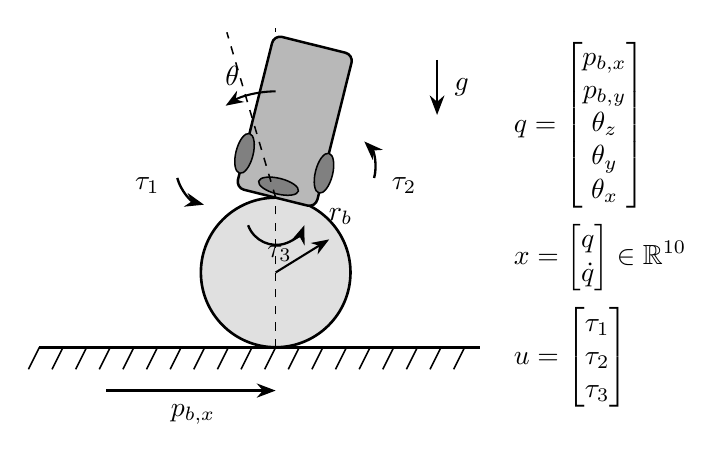
\begin{tikzpicture}[
  >=Stealth,
  font=\normalsize
]
  % ground
  \draw[line width=0.95pt] (-3.0,0) -- (2.6,0);
  \foreach \x in {-3.0,-2.7,...,2.5}
    \draw[line width=0.55pt] (\x,0) -- ++(-0.14,-0.28);

  % ball
  \coordinate (B) at (0,0.95);
  \filldraw[fill=black!12, draw=black, line width=0.95pt] (B) circle (0.95);
  \draw[->, line width=0.75pt] (B) -- ($(B)+(0.68,0.42)$);
  \node[anchor=south west] at ($(B)+(0.55,0.48)$) {$r_b$};

  % vertical reference through contact
  \draw[dashed, line width=0.5pt] (0,0) -- (0,4.05);

  % body (tilted about contact with ball top)
  \coordinate (Pivot) at (0,1.90);
  \begin{scope}[rotate around={-14:(Pivot)}]
    \filldraw[fill=black!28, draw=black, line width=0.9pt, rounded corners=3pt]
      (-0.52,1.90) rectangle (0.52,3.90);
    % three omniwheels at ball–body interface
    \filldraw[fill=black!50, draw=black, line width=0.55pt]
      (-0.52,2.35) ellipse (0.11 and 0.26);
    \filldraw[fill=black!50, draw=black, line width=0.55pt]
      (0.52,2.35) ellipse (0.11 and 0.26);
    \filldraw[fill=black!50, draw=black, line width=0.55pt]
      (0,2.05) ellipse (0.26 and 0.10);
  \end{scope}

  % lean: body axis + angle arc
  \draw[dashed, line width=0.55pt] (0,1.90) -- (-0.62,4.0);
  \draw[->, line width=0.75pt] (0,3.25) arc (90:122:1.20);
  \node at (-0.55,3.45) {$\theta$};

  % planar position
  \draw[->, line width=0.85pt] (-2.15,-0.55) -- (0,-0.55);
  \node[anchor=north] at (-1.05,-0.60) {$p_{b,x}$};

  % wheel torques (all three with arcs)
  \draw[->, line width=0.85pt] (-1.25,2.15) arc (195:255:0.48);
  \node[anchor=east] at (-1.35,2.05) {$\tau_1$};
  \draw[->, line width=0.85pt] (1.25,2.15) arc (-15:45:0.48);
  \node[anchor=west] at (1.35,2.05) {$\tau_2$};
  \draw[->, line width=0.85pt] (-0.35,1.55) arc (200:340:0.38);
  \node[anchor=north] at (0.05,1.42) {$\tau_3$};

  % gravity
  \draw[->, line width=0.9pt] (2.05,3.65) -- (2.05,2.95);
  \node[anchor=west] at (2.15,3.30) {$g$};

  % equations (DI layout: north-west block)
  \node[anchor=north west, align=left] at (2.9,4.0) {%
    $\displaystyle q=\begin{bmatrix}p_{b,x}\\ p_{b,y}\\ \theta_z\\ \theta_y\\ \theta_x\end{bmatrix}$\\[5pt]
    $\displaystyle x=\begin{bmatrix}q\\ \dot{q}\end{bmatrix}\in\mathbb{R}^{10}$\\[5pt]
    $\displaystyle u=\begin{bmatrix}\tau_1\\ \tau_2\\ \tau_3\end{bmatrix}$%
  };
\end{tikzpicture}
\end{document}
